\section{External World Interfaces \embsys{383}{8}}
\subsection{General Purpose Input-Output Ports (GPIO) \embsys{383}{8.1}}
\subsubsection{General Characteristics of I/O Ports}
\begin{itemize}
	\item Allow comunication with the external world
	\item Operate digitally and can be configured as either inputs or outputs
	\item Can be configured individually or in groups called ports
\end{itemize}
CodeBSP siehe Anhang \label{GPIO}
\begin{multicols}{2}
	\subsubsection{Structure of an Input-Output Pin \embsys{384}{8.1.1}}
	\begin{itemize}
		\item Input Pins, for binary Status
		\item Output Pins, for binary Status
		\item \acs{GPIO} Interfaces, for General IN or OUT
	\end{itemize}	
	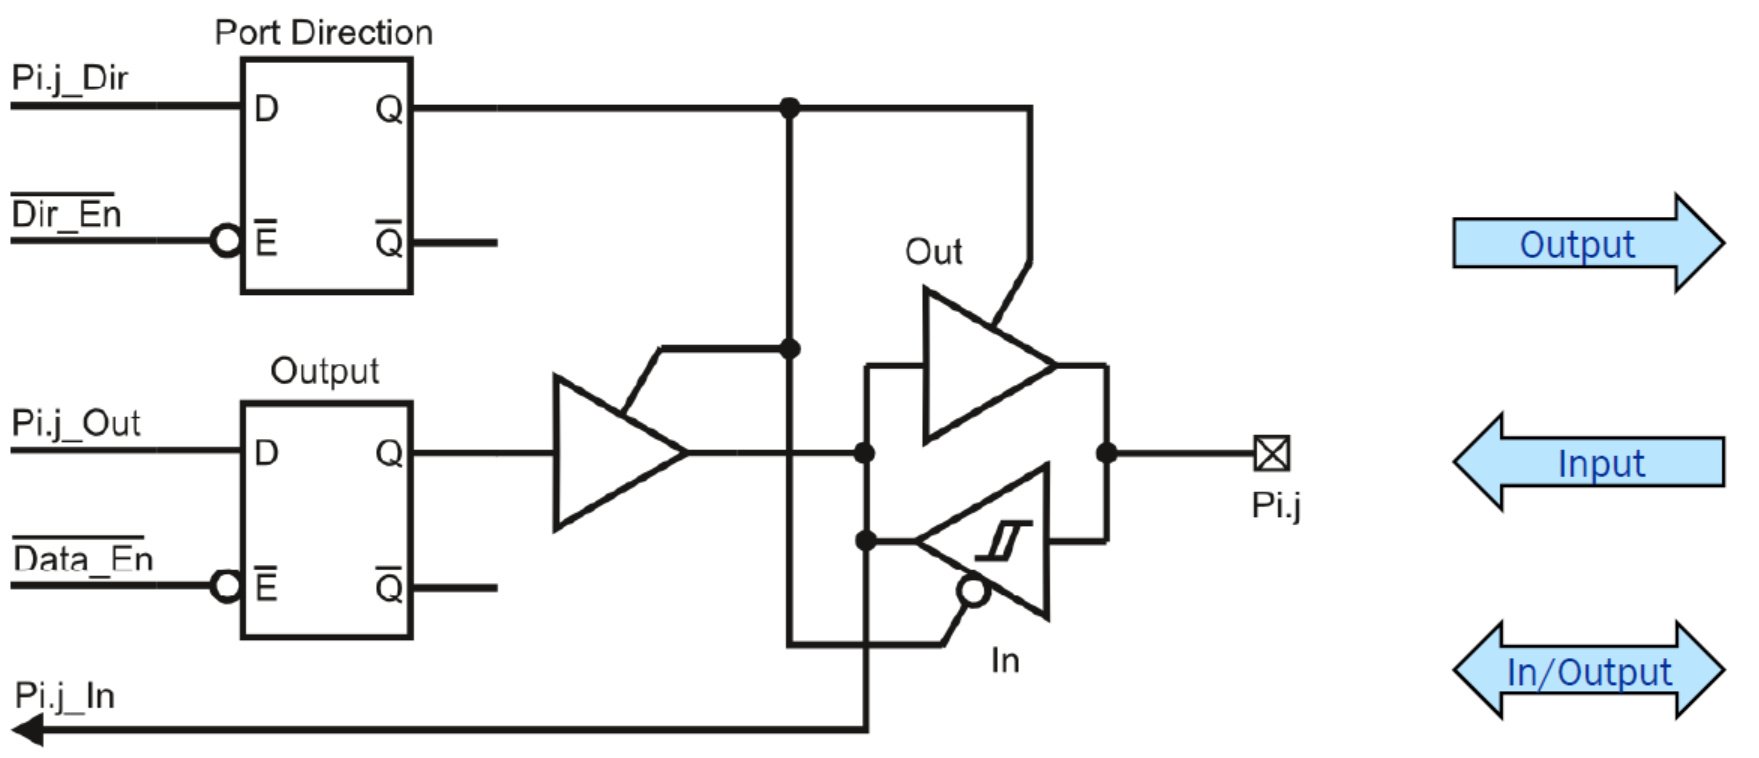
\includegraphics[width=\linewidth]{images/IOStructure}  
\end{multicols}

\subsubsection{MSP430 GPIO Registers \embsys{388}{8.1.3}}
\begin{tabular}{>{\bfseries}lll}
	PxSEL   &Port x Function Select             & Sets pin functionality  \\ 
	PxDIR   &Port x Data Direction              & Sets pin as either IN or OUT \\ 
	PxOut   &Port x Out                         & Data-out register \\ 
	PxIN    &Port x Input                       & Data-in register  \\ 
	PxIFG   &Port x Interrupt Flag              & Interrupt request for port x \\ 
	PxIES   &Port x Interrupt Edge Selection    & Sets signal edge to trigge interrupts in Port x input  \\ 
	PxIE    &Port x Interrupt Enable            & Enables interrupts from Port x pins \\ 
	PxREN   &Port x Ressistor Enable            & Enables internal pull-up/down resistors \\ 
	PxDS    &Port x Drive Strength              & Sets driver strength for port pins to up to 30mA  \\ 
	PxIV    &Port x Interrupt Vector            & Priority encoding for port Interrupts \\ 
\end{tabular} 

\subsubsection{Electrical Characteristics in I/O Pins \embsys{391}{8.2.1}}
\begin{tabular}{lll}
	$ V_{IL} $& Input Low Voltage&Maximum voltage inperpreted as low by pin input buffer\\
	$ V_{IH} $& Input High Voltage& Minimum voltage interpreted as high by pin input buffer\\
	$ V_{OL} $& Output Low Voltage& Locig-low level. Minimum voltage oserved at pin outputdriver\\
	$ V_{OH} $& Output High Voltage& Logic-high level. Maximum voltage observed at pin output driver\\
	$ V_M $   & Pin Threshold Voltage& Ultimate level seperating low and high levels in a digital pin\\
	&                      & Specified as $ V_m=V_{DD}/2 $ for CMOS logic\\
\end{tabular} 
\clearpage
%=========================================

\subsection{Interfacing Switches and Switch Arrays \embsys{402}{8.3}}
\subsubsection{Switches and Buttons}
	Mechanical Contact with two States (Open, Closed). Each State of the Switches has to translate into a Valid Logic Level. 
	\begin{itemize}
		\item \textbf{Pull-Down}
		\subitem Pull-down bezeichnet einen hochohmigen Widerstand, der eine Signalleitung mit dem niedrigeren Spannungs-Potential verbindet. Durch ihn wird die Leitung auf das niedrige Potential gebracht, für den Fall, dass kein Ausgang die Leitung aktiv auf ein höheres Potential bringt.
		\item \textbf{Pull-Up}
		\subitem Pull-up bezeichnet einen hochohmigen Widerstand, der eine Signalleitung mit dem höheren Spannungs-Potential verbindet. Durch ihn wird die Leitung auf das höhere Potential gebracht, für den Fall, dass kein Ausgang die Leitung aktiv auf ein niedrigeres Potential bringt.
	\end{itemize}
	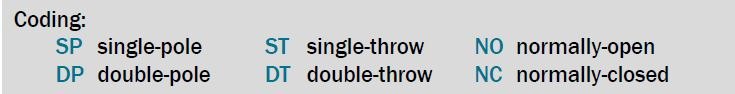
\includegraphics[width=0.6\linewidth]{images/Coding_SW_BT.jpg}
\begin{multicols}{2}
	\textbf{Switches}\\
	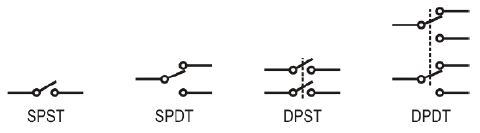
\includegraphics[width=0.6\linewidth]{images/Switches.jpg}\\
	\textbf{Momentary Push Buttons}\\
	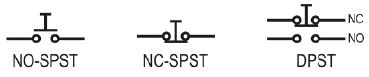
\includegraphics[width=0.6\linewidth]{images/Buttons.jpg}
\end{multicols}
\subsubsection{Switch Arrays and Keypads}
\begin{multicols}{2}
	\begin{itemize}
		\item \textbf{Switch Arrays}
		\subitem Contains 2 to 8 SPST Switches
		\subitem Interfaced individually
		\subitem Interpreted as a whole number
		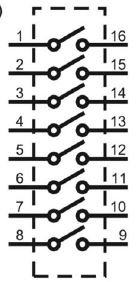
\includegraphics[width=0.3\linewidth]{images/Switch_Array.jpg}  
		\item \textbf{Keypads}
		\subitem Matrix Switch Arrays
		\subitem Interfaced via rwo-column arragement
		\subitem Interpreted as a scan-return code 
		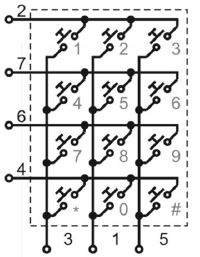
\includegraphics[width=0.5\linewidth]{images/Keypad.jpg}
	\end{itemize}
\end{multicols}
\subsubsection{Hardware Debouncing Techniques \embsys{407}{8.3.7}}
\begin{multicols}{2}
    \begin{itemize}
        \item Reduce software complexity
        \item Increase components on board
    \end{itemize}
\end{multicols}
\textbf{Set-Reset Debouncing Circuit}\newline
\begin{minipage}{0.5\linewidth}
    \begin{itemize}
        \item Will debounce regardless of its bounce time
        \item R1 and R2 are Pull-Ups
        \item SW1 needs to be a SPDT switch.
    \end{itemize}
\end{minipage}
\begin{minipage}{0.5\linewidth}
    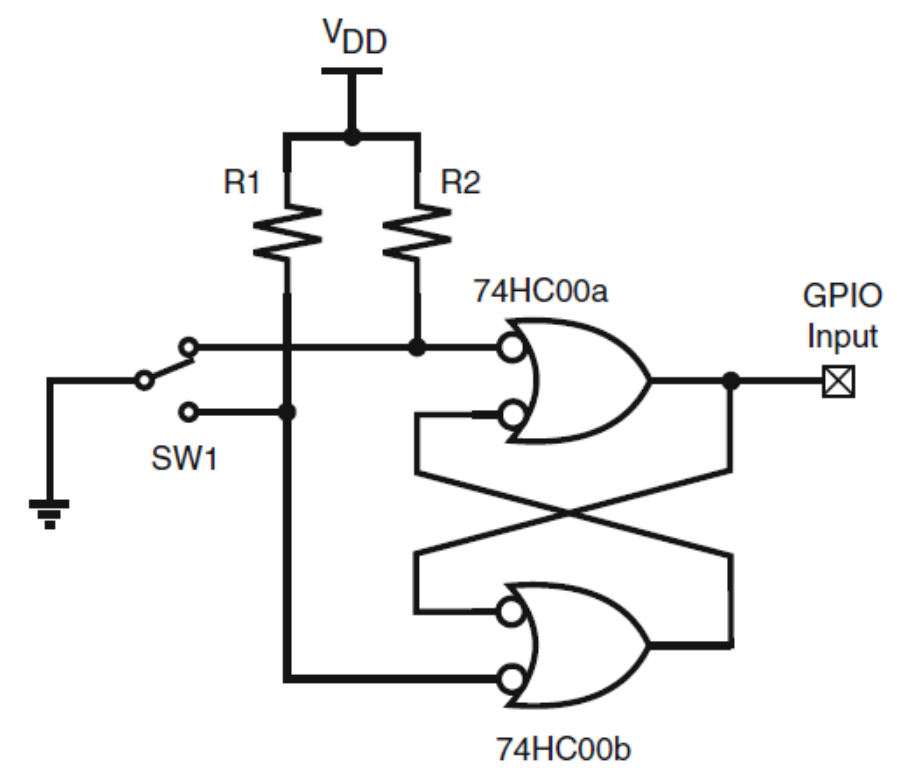
\includegraphics[width=0.5\linewidth]{images/HWDebounceSR}  
\end{minipage}

\textbf{RC Debouncing Circuit}\newline
\begin{minipage}{0.5\linewidth}
    \begin{itemize}
        \item cost effective
    \end{itemize}
    \[ V_x = V_{DD}\cdot e^{-(\frac{t_{bounce}}{R_2 C_1})} \]
    \[ (R_1 + R_2) \geq \frac{t_{bounce}}{C_1 \cdot ln(\frac{V_{DD}}{V_{DD}-V_T^+})} \]
\end{minipage}
\begin{minipage}{0.5\linewidth}
    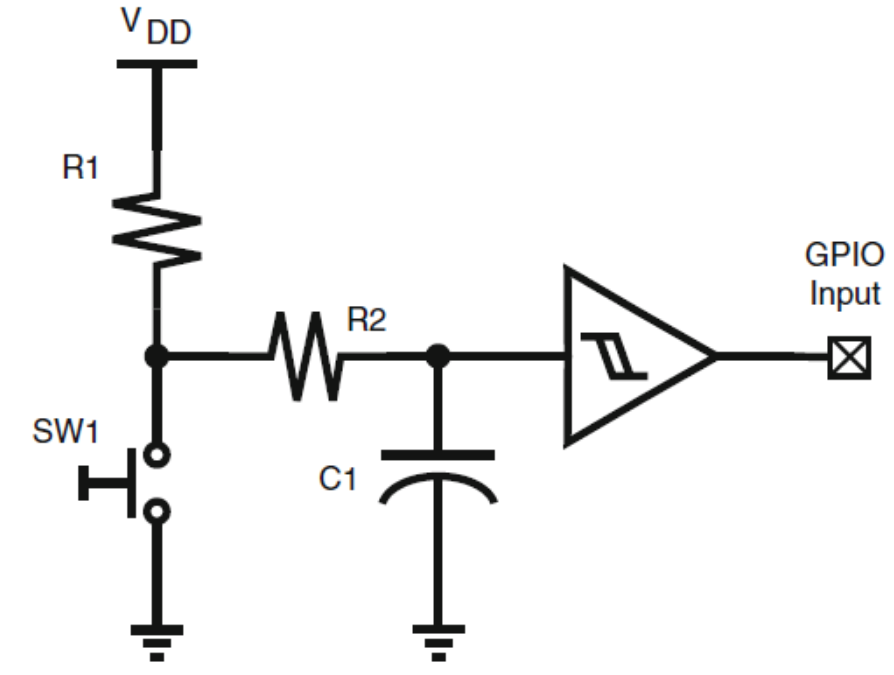
\includegraphics[width=0.5\linewidth]{images/HWDebounceRC}  
\end{minipage}

\textbf{IC Debouncing Circuit}\newline
\begin{minipage}{0.5\linewidth}
    \begin{itemize}
        \item Convenient for debouncing multiple switches
    \end{itemize}
    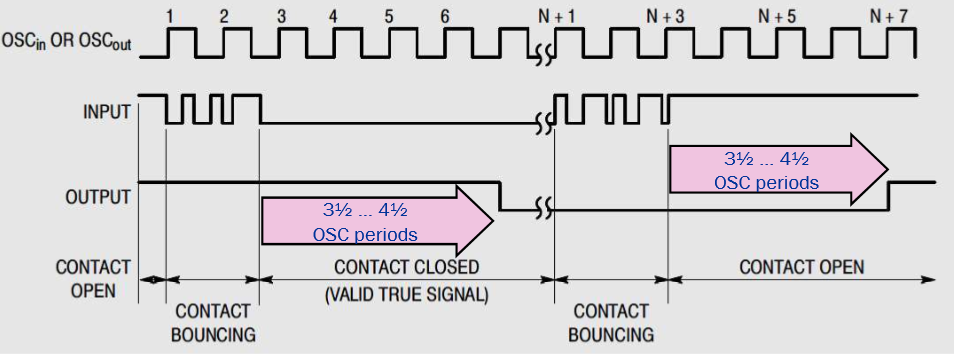
\includegraphics[width=0.8\linewidth]{images/HWDebounceICTiming}  
\end{minipage}
\begin{minipage}{0.5\linewidth}
    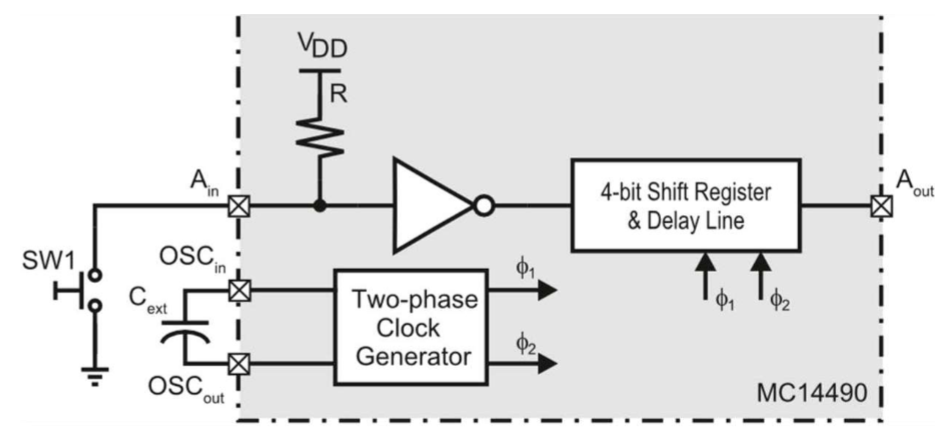
\includegraphics[width=0.9\linewidth]{images/HWDebounceIC}  
\end{minipage}
\subsubsection{Software Debouncing Techniques \embsys{410}{8.3.8}}
\begin{multicols}{2}
\textbf{Recommendations}
\begin{itemize}
    \item Avoid waisting cycles while waiting for bouncing end.
        \subitem Use Low Power Mode instead
    \item Keep SW respones short
        \subitem Most switch bounce less than 15ms.
    \item Humans can detect response delays with 75ms
\end{itemize}
\columnbreak
\textbf{Solutions}
\begin{itemize}
    \item Remove Switch Transient via Time Delays
        \subitem consumes \acs{CPU} cycles
    \item Polling Debouncer
        \subitem Pol the switch with $ t_{poll} > t_{bounce} $
    \item Counting Debouncer
        \subitem Assumes switch has settled when no bounce is detected for n samples
        \subitem If a bounce were detected bofore n, the counter restarts 
        \subitem Siehe CodeBSP in Anhang \label{CountingDebouncer}     
\end{itemize}
\end{multicols}
\subsection{Interfacing LEDs}
\begin{itemize}
	\item Discrete \acs{LED}s
	\subitem Requires a current and driving circuit
	\item Numeric Display (Seven-Segment Modules)
	\subitem Array of 7 bar-shaped \acs{LED} forms digits from 0 to 9
	\subitem Each digit needs to be refreshed at 24 Hz
	\item Alphanumeric Displays
	\subitem Able to produce numbers and alphabetic characters
	\item Graphic Panels
	\subitem Pixel addressable Panels
\end{itemize}
\subsection{Interfacing \acs{LCD}s}
\begin{itemize}
	\item Liquid Crystal Displays (\acs{LCD}) use the property of liquid crystal materials of twisting the polarization angle of coherent light
	\item Thin Film Transistor (\acs{TFT}) uses row column cell
\end{itemize}
\clearpage